\section{Опис програмної моделі}

При виконанні лабораторних робіт і курсового проекту був розроблений програмний продукт для аналізу алгоритмів планування для MPP систем.

\subsection{Загальна організація програми}
    Програма розроблена мовою Python з використанням графічної бібліотеки Tkinter. Для виводу діаграм Ганта використовувалася бібліотека matplotlib для побудови діаграм.

    Інтрфейс користувача для вводу графу задачі показаний на рис. \ref{fig:gui}.
    \begin{figure}[h!]
      \begin{center}
        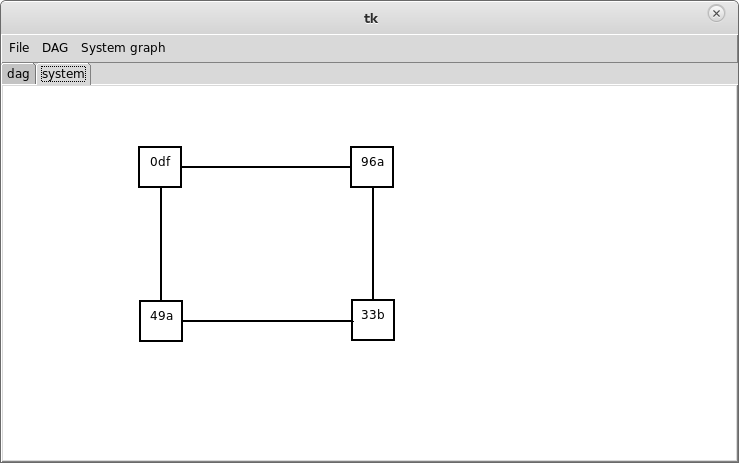
\includegraphics[width=\textwidth]{res/system_graph.png}
      \end{center}
      \caption{Інтерфейс користувача}
    \label{fig:gui}
    \end{figure}

\subsection{Внутрішнє представлення системи}
    Система представлена як група процесорів із заданою кількістю лінків. Система представлена класом System, він інкапсулює процесори, що представлені класом CPU, що також інкапсулює лінки (клас Link). Кожен процесор та лінк має можливість зберігати часові проміжки ScheduledTransmissionSegment та ScheduledTask, що репрезентують сегмент пересилання даних та сегмант обрахунку задачі відповідно.

Алгоритм перевірки на зв'язність: запускається алгоритм пошуку в глибину починаючи від першої вершини. Якщо пройдені вершини містять всі вершини графа, то граф зв'язний. Інтрфейс користувача для вводу графу системи показаний на рис. \ref{fig:system_graph}.
    \begin{figure}[h!]
      \begin{center}
        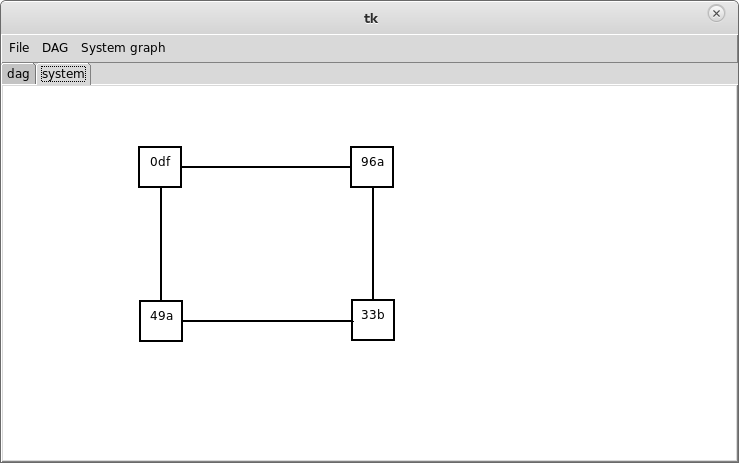
\includegraphics[width=\textwidth]{res/system_graph.png}
      \end{center}
      \caption{Інтерфейс користувача вводу задачі}
    \label{fig:system_graph}
    \end{figure}



    Для представлення графу задачі використовується кореневий клас DAG, що зберігає вершини у класах Node та зв'язки між ними у класах Edge.

    Алгоритм перевірки на ациклічності: запускається алгоритм пошуку в глибину починаючи від кожної вершини, генеруючи дерево вершин з коренем в поточній. Якщо в це дерево потрапляє вершина, яка вже в ньому присутня, то знайдений цикл. Інтрфейс користувача для вводу графу задачі показаний на рис. \ref{fig:gui_graph}.
    \begin{figure}[h!]
      \begin{center}
        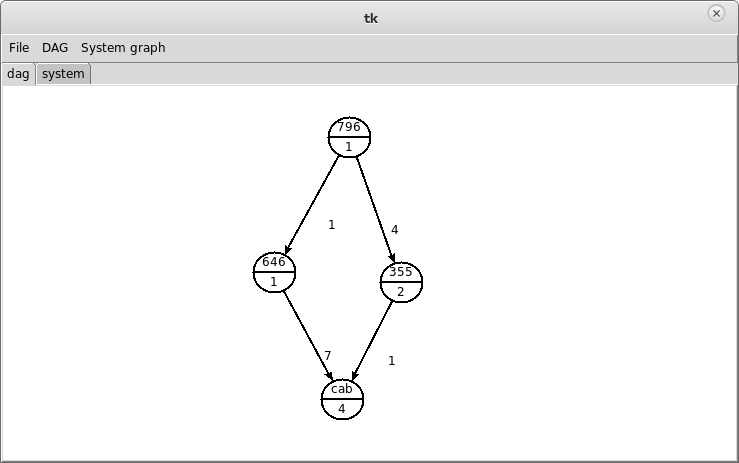
\includegraphics[width=\textwidth]{res/gui_graph.png}
      \end{center}
      \caption{Інтерфейс користувача вводу задачі}
    \label{fig:gui_graph}
    \end{figure}


\subsection{Алгоритми формування черги}
Алгоритми формування черги інкапсулюються в нащадків класу BaseQueueGenerationPolicy, в яких має бути реалізований метод get\_queue.

Алгоритм 3 формує чергу у порядку спадання критичного по часу шляхів до кінця графа задачі. Програма формує всі критичні шляхи у графі задачі і сортує їх за часом. Якщо час однаковий, то за номером вершини. Реалізація алгоритму у алгоритмі \ref{lst:a3}.

\begin{lstlisting}[language=Python,caption={Алгоритм 3},label=lst:a3]
class QueueGenerationPolicy3(BaseQueueGenerationPolicy):
    def get_queue(self, dag):
        paths = find_all_critical_paths(dag, forward=True, weight_based=True)

        def get_weight(item):
            node_id, (weight, path) = item
            return weight, node_id
        return [path[0] for path in sorted(paths.items(), key=get_weight, reverse=True)]

\end{lstlisting}

Алгоритм 4 формує чергу у порядку спадання критичного по кількості вершин шляхів до кінця графа задачі, а при рівних значеннях – в порядку спадання зв’язності вершин. Необхідно визначити всі критичні шляхи за кількістю вершин та відсортувати за кількістю, а при рівних - в спаданні зв'язності.  Реалізація алгоритму у алгоритмі \ref{lst:a4}.

\begin{lstlisting}[language=Python,caption={Алгоритм 4},label=lst:a4]
class QueueGenerationPolicy4(BaseQueueGenerationPolicy):
    def get_queue(self, dag):
        paths = find_all_critical_paths(dag, forward=True, weight_based=False)

        def get_weight(item):
            node_id, (weight, path) = item
            node = dag.nodes[node_id]
            return weight, len(dag.get_neighbours(node, forward=True) + dag.get_neighbours(node, forward=False))
        return [path[0] for path in sorted(paths.items(), key=get_weight, reverse=True)]

\end{lstlisting}

Алгоритм 16 формує чергу у порядку зростання критичного по часу шляхів вершин від початку графа задачі. Необхідно визначити критичні шляхи від початку графу та відсортувати за часом. Реалізація алгоритму у алгоритмі \ref{lst:a16}.

\begin{lstlisting}[language=Python,caption={Алгоритм 16},label=lst:a16]
class QueueGenerationPolicy16(BaseQueueGenerationPolicy):
    def get_queue(self, dag):
        paths = find_all_critical_paths(dag, forward=False, weight_based=True)

        def get_weight(item):
            node_id, (weight, path) = item
            return weight
        return [path[0] for path in sorted(paths.items(), key=get_weight)]

\end{lstlisting}

\subsection{Генерация випадкового графу задачі}    

Необхідно сформувати випадковий граф задачі за заданими параметрами. Програма надає можливість задання таких параметрів: (див. рис. \ref{fig:random_params})

    \begin{figure}[h!]
      \begin{center}
        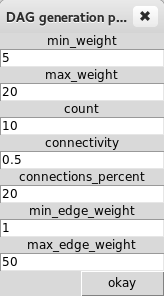
\includegraphics{res/random.png}
      \end{center}
      \caption{Інтерфейс задання параметрів випадкової задачі}
    \label{fig:random_params}
    \end{figure}

Алгоритм генерації випадкового графу:

\begin{enumerate}
    \item Генеруємо N вершин з випадковими вагами в заданих межах.
    \item Рахуємо суму вагів, за формулою кореляции рахуємо середню вагу дуги яку ми повинні отримати.
    \item По заданому відсотку кількості дуг та середному значенню, рахуємо їх кількість і генеруємо їх.
    \item Ваги дуг задаємо випадковим чином по нормальному розподілу, де mu = (очікувана сума) / (кількість дуг), а sigma = mu / 4, при цьому не дозволяємо вазі виходити за задані межі. При цьому, якщо середнє значення виходить за межі, то межі не враховуються.
    \item Якщо потрібна кореляція досягнута, але не всі ребра додані, зупиняємо додавання ребер.
    \item В останню дугу вагою записуємо необхідну різницю, щоб отримати потрібний коефіцієнт кореляції - без урахування меж.
\end{enumerate}

\begin{lstlisting}[language=Python,caption={Вихідний код генерації випадкового графу задачі},label=lst:random_dag]
    def generate(cls,
                 min_weight, max_weight,
                 count, connectivity, connections_percent,
                 min_edge_weight=None, max_edge_weight=None):
        graph = DAG()
        sum_weight = 0
        for i in range(count):
            weight = randint(min_weight, max_weight)
            graph.add_node(randint(0, 300), randint(0, 300), weight, str(i))
            sum_weight += weight

        sum_edges_weight = (sum_weight - connectivity*sum_weight) / connectivity

        max_edges_count = (count*(count-1)) / 2
        edges_count = int(connections_percent/100*max_edges_count)

        pairs = [(str(i), str(j)) for i in range(count) for j in range(i+1, count)]
        # 1 1 30 0.1 10 1 500
        sum_edges_weight_actual = 0
        last_edge = None
        added_edges_count = 0
        for source, target in sample(pairs, edges_count):
            average_edge_weight = max(1, ((sum_edges_weight - sum_edges_weight_actual) / (edges_count - added_edges_count)))
            weight = int(normalvariate(average_edge_weight, average_edge_weight/4))
            weight = norm_weight(weight, min_edge_weight, max_edge_weight, average_edge_weight)
            if sum_edges_weight - (sum_edges_weight_actual + weight) < 0:
                weight = max(1, int(sum_edges_weight - sum_edges_weight_actual))
                last_edge = graph.add_edge(source, target, weight)
                sum_edges_weight_actual += weight
                warnings.warn("Stopped, maximum reached: last edge weight was {} < {} < {}".
                              format(min_edge_weight, weight, max_edge_weight))
                break
            last_edge = graph.add_edge(source, target, weight)
            sum_edges_weight_actual += weight
            added_edges_count += 1
        else:
            weight = int(sum_edges_weight - sum_edges_weight_actual)
            if weight <= 0:
                weight = 1
            last_edge.weight = weight
            expected_weight = norm_weight(weight, min_edge_weight, max_edge_weight, average_edge_weight)
            if expected_weight != weight:
                warnings.warn("Last edge weight was out of bounds {} < {} < {}".
                              format(min_edge_weight, weight, max_edge_weight))

        graph.arrange()
        print("Correlation")
        print("actual: ", graph.correlatio(), "; expected: ", connectivity)
        return graph


\end{lstlisting}


\subsection{Процесс моделирования}

TODO!!!!!!!!!!!!!!!!!!!!!!!!!!!!!!!!!!!!!!!!!!!!!!!!!!!!
TODO!!!!!!!!!!!!!!!!!!!!!!!!!!!!!!!!!!!!!!!!!!!!!!!!!!!!
TODO!!!!!!!!!!!!!!!!!!!!!!!!!!!!!!!!!!!!!!!!!!!!!!!!!!!!
TODO!!!!!!!!!!!!!!!!!!!!!!!!!!!!!!!!!!!!!!!!!!!!!!!!!!!!
TODO!!!!!!!!!!!!!!!!!!!!!!!!!!!!!!!!!!!!!!!!!!!!!!!!!!!!
TODO!!!!!!!!!!!!!!!!!!!!!!!!!!!!!!!!!!!!!!!!!!!!!!!!!!!!
TODO!!!!!!!!!!!!!!!!!!!!!!!!!!!!!!!!!!!!!!!!!!!!!!!!!!!!
TODO!!!!!!!!!!!!!!!!!!!!!!!!!!!!!!!!!!!!!!!!!!!!!!!!!!!!
TODO!!!!!!!!!!!!!!!!!!!!!!!!!!!!!!!!!!!!!!!!!!!!!!!!!!!!

\subsection{Інструкція користувача}

Користувачу достіпні два екрани для вводу графів задачі (рис. \ref{fig:gui_graph_2}) та системи (рис. \ref{fig:system_graph_2}).

    \begin{figure}[h!]
      \begin{center}
        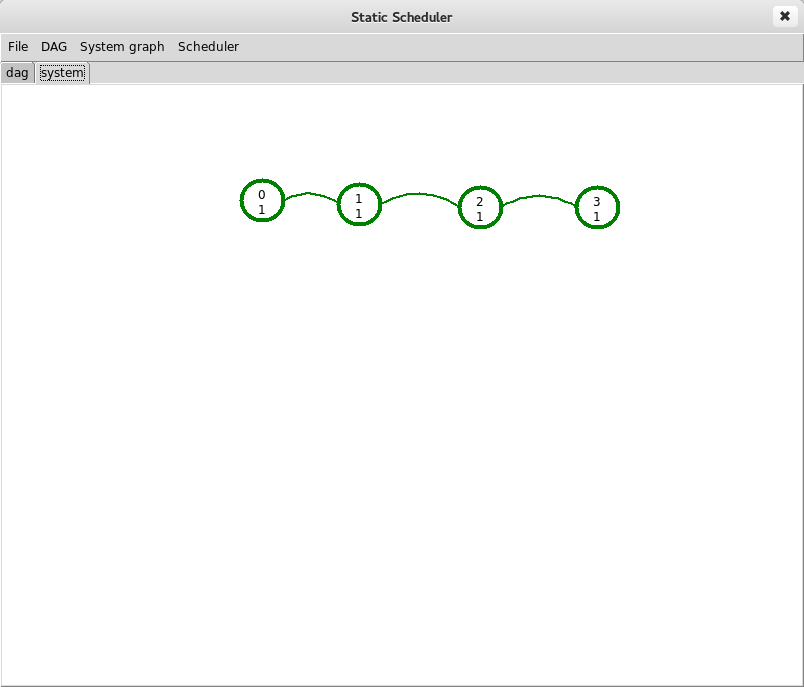
\includegraphics[width=\textwidth]{res/system_graph_new.png}
      \end{center}
      \caption{Інтерфейс користувача вводу задачі}
    \label{fig:system_graph_2}
    \end{figure}

    \begin{figure}[h!]
      \begin{center}
        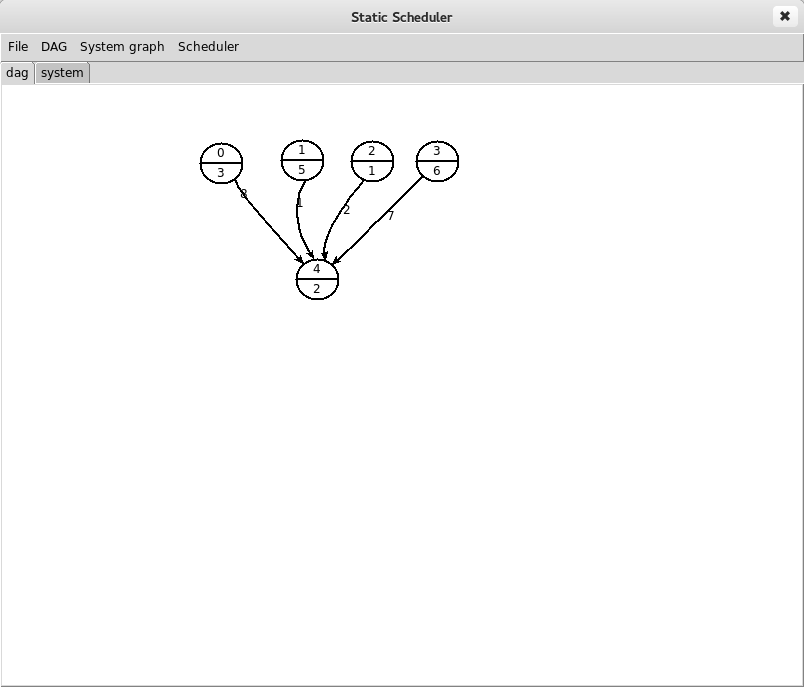
\includegraphics[width=\textwidth]{res/gui_graph_new.png}
      \end{center}
      \caption{Інтерфейс користувача вводу задачі}
    \label{fig:gui_graph_2}
    \end{figure}

Можливе зберігання та відкриття збережених графів задач та систем через меню File.

Для запуску процесу планування використовується пункт меню Scheduler -> Schedule.
Налаштування планувальника на рис. \ref{fig:sched_params}

    \begin{figure}[h!]
      \begin{center}
        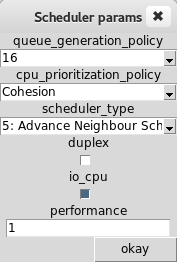
\includegraphics{res/sched_params.png}
      \end{center}
      \caption{Налаштування планувальника}
    \label{fig:sched_params}
    \end{figure}
